\documentclass[t,aspectratio=169]{beamer} % 使用16:9宽高比
\usetheme{Madrid} % 选择Madrid主题
\usecolortheme{default} % 使用默认颜色主题

% 设置字体
\usepackage[UTF8]{ctex}
\usefonttheme{structurebold} % 加粗结构字体

% 数学包
\usepackage{amsmath, amssymb, bm}
\usepackage{url}
\usepackage{booktabs}

% 图形包
\usepackage{graphicx}

% 标题页信息
\title[9.6.模型平均]{第9章：正则化}
\subtitle{第6节：模型平均 (Model Averaging)}
\author{《深度学习基础》课程小组}
% \institute{上海立信会计金融学院}
\date{\today}

\begin{document}

% 标题页
\frame{\titlepage}

% 目录页
\begin{frame}
    \frametitle{目录}
    \tableofcontents
\end{frame}

% ============================================================
% 第一部分：集成方法
% ============================================================
\section{集成方法}

\begin{frame}
    \frametitle{1. 集成方法 (Ensembles)}
    \begin{itemize}
        \item 若有多个不同模型解决同一问题，\alert{平均预测}往往比选择单个最佳模型更好。
        \item 这种模型组合称为\alert{委员会}或\alert{集成}。
        \item 对产生概率输出的模型，预测分布为各模型预测的平均：
        \begin{equation}
            p(\mathbf{y}|\mathbf{x}) = \frac{1}{L} \sum_{l=1}^{L} p_l(\mathbf{y}|\mathbf{x})
            \tag{9.42}
        \end{equation}
        \item 平均过程的动机：\alert{偏差-方差权衡}。
        \begin{itemize}
            \item 多个多项式在正弦数据上训练后平均，方差项趋于\alert{抵消}，改善预测。
        \end{itemize}
    \end{itemize}
\end{frame}

\begin{frame}
    \frametitle{1.1 自助聚合 (Bagging)}
    \begin{itemize}
        \item \textbf{实际问题}：只有一个数据集，需要引入模型间的\alert{变异性}。
        \item \textbf{自助数据集}（bootstrap）：
        \begin{itemize}
            \item 从原始数据集 $\mathbf{X} = \{\mathbf{x}_1, \ldots, \mathbf{x}_N\}$ 中\alert{有放回}地抽取 $N$ 个点。
            \item 某些点可能被重复，某些点可能缺失。
        \end{itemize}
        \item 重复 $L$ 次生成 $L$ 个数据集，每个训练一个模型，预测取平均。
        \item 该过程称为\alert{自助聚合}或\alert{bagging} (Breiman, 1996)。
        \item \textbf{替代方法}：用原始数据集训练多个\alert{不同架构}的模型。
    \end{itemize}
\end{frame}

\begin{frame}[allowframebreaks]
    \frametitle{1.2 集成预测的理论分析}
    考虑回归问题，集成预测：
    \begin{equation}
        y_{\text{COM}}(\mathbf{x}) = \frac{1}{M} \sum_{m=1}^{M} y_m(\mathbf{x})
        \tag{9.43}
    \end{equation}
    每个模型输出 = 真实值 + 误差：
    \begin{equation}
        y_m(\mathbf{x}) = h(\mathbf{x}) + \epsilon_m(\mathbf{x})
        \tag{9.44}
    \end{equation}
    平均误差：
    \begin{equation}
        E_{\text{AV}} = \frac{1}{M} \sum_{m=1}^{M} \mathbb{E}_{\mathbf{x}} \left[ \epsilon_m(\mathbf{x})^2 \right]
        \tag{9.46}
    \end{equation}
    集成误差（假设误差零均值且\alert{不相关}）：
    \begin{equation}
        E_{\text{COM}} = \frac{1}{M} E_{\text{AV}}
        \tag{9.50}
    \end{equation}
    \begin{itemize}
        \item \alert{戏剧性结果}：平均可将误差降低 $M$ 倍。
        \item \textbf{但关键假设}：各模型误差\alert{不相关}。
        \item 实践中误差高度相关，实际降低幅度小得多。
        \item 但可证明：$E_{\text{COM}} \leq E_{\text{AV}}$。
    \end{itemize}
\end{frame}

\begin{frame}
    \frametitle{1.3 Boosting：提升方法}
    \begin{itemize}
        \item 另一种模型组合方法：\alert{boosting} (Freund and Schapire, 1996)。
        \item 组合多个\alert{基分类器}，性能可显著优于任何单个基分类器。
        \item 即使基分类器仅比随机猜测稍好，boosting 也能给出好结果。
    \end{itemize}
    \begin{block}{与 Bagging 的关键区别}
        \begin{itemize}
            \item 基分类器\alert{按顺序训练}。
            \item 每个基分类器使用\alert{加权形式}的数据集。
            \item 权重取决于\alert{前一个分类器的表现}。
            \item 被前一个分类器\alert{误分类}的点在训练下一个分类器时获得\alert{更大权重}。
            \item 最终通过\alert{加权多数投票}组合预测。
        \end{itemize}
    \end{block}
\end{frame}

\begin{frame}
    \frametitle{1.4 模型组合的主要缺点}
    \begin{itemize}
        \item \textbf{所有模型组合方法的主要缺点}：
        \begin{itemize}
            \item 需训练多个模型。
            \item 需为所有模型评估预测。
            \item 增加\alert{训练和推理}的计算成本。
        \end{itemize}
        \item 严重程度取决于具体应用场景。
    \end{itemize}
\end{frame}

% ============================================================
% 第二部分：Dropout
% ============================================================
\section{Dropout}

\begin{frame}[allowframebreaks]
    \frametitle{2. Dropout：隐式模型平均}
    \begin{itemize}
        \item 广泛使用且非常有效的正则化形式 (Srivastava et al., 2014)。
        \item 可视为对\alert{指数级多个模型}进行近似模型平均的\alert{隐式方法}。
        \item 无需单独训练多个模型。
        \item 适用性广，计算成本低。
        \item 是最有效的正则化形式之一，应用广泛。
    \end{itemize}
    \begin{block}{核心思想}
        训练时\alert{随机删除}网络中的节点（包括其连接）。\\
        每次呈现数据点时，重新随机选择要省略的节点。
    \end{block}
    \begin{figure}
        \centering
        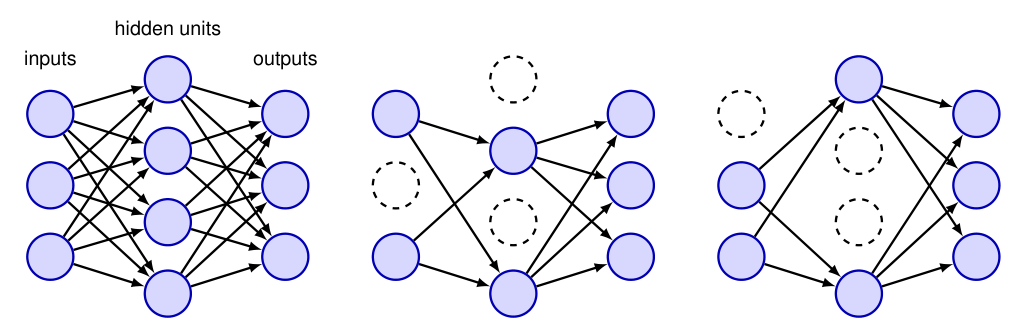
\includegraphics[width=0.45\textwidth]{figure-9-17.png}
        \caption{原始网络（左）和两个剪枝网络示例（右）。}
    \end{figure}
\end{frame}

\begin{frame}
    \frametitle{2.1 Dropout 的实现}
    \begin{itemize}
        \item 应用于\alert{隐藏节点和输入节点}，但\alert{不应用于输出节点}。
        \item 等价于将丢弃节点的输出设为\alert{零}。
        \item 实现：定义\alert{掩码向量} $R_i \in \{0, 1\}$。
        \begin{itemize}
            \item 乘以非输出节点 $i$ 的激活值。
            \item 值为 1 的概率为 $\rho$。
        \end{itemize}
        \item \textbf{典型值}：
        \begin{itemize}
            \item 隐藏节点：$\rho = 0.5$
            \item 输入节点：$\rho = 0.8$
        \end{itemize}
    \end{itemize}
\end{frame}

\begin{frame}
    \frametitle{2.2 Dropout 的训练过程}
    \begin{itemize}
        \item 每个数据点呈现时，创建\alert{新掩码}。
        \item 在剪枝网络上应用前向和反向传播，创建误差函数梯度。
        \item 用梯度更新权重（如 SGD）。
        \item 小批量：梯度在小批量内平均后再更新权重。
        \item 有 $M$ 个非输出节点的网络有 $2^M$ 个剪枝网络。
        \begin{itemize}
            \item 训练中只考虑其中\alert{一小部分}。
        \end{itemize}
    \end{itemize}
    \begin{block}{与传统集成方法的区别}
        \begin{itemize}
            \item 传统集成：每个网络\alert{独立训练至收敛}。
            \item Dropout：隐含训练的指数级多个网络\alert{不独立}，而是与完整网络\alert{共享参数}。
        \end{itemize}
    \end{block}
\end{frame}

\begin{frame}
    \frametitle{2.3 Dropout 的注意事项}
    \begin{itemize}
        \item \alert{训练时间可能更长}：
        \begin{itemize}
            \item 单个参数更新\alert{非常嘈杂}。
        \end{itemize}
        \item \alert{误差函数本质上是嘈杂的}：
        \begin{itemize}
            \item 更难通过观察误差函数下降来确认优化算法正常工作。
        \end{itemize}
    \end{itemize}
\end{frame}

\begin{frame}
    \frametitle{2.4 推理阶段：模型平均}
    训练完成后，原则上可用集成规则 (9.42)：
    \begin{equation}
        p(\mathbf{y}|\mathbf{x}) = \sum_{\mathbf{R}} p(\mathbf{R}) p(\mathbf{y}|\mathbf{x}, \mathbf{R})
        \tag{9.51}
    \end{equation}
    \begin{itemize}
        \item 求和遍历\alert{指数级大的掩码空间}。
        \item 该求和\alert{难以处理}，可通过采样少量掩码近似。
        \item 实践中\alert{10 到 20 个掩码}即可获得良好结果。
        \item 该过程称为\alert{蒙特卡洛 Dropout}。
    \end{itemize}
    \begin{block}{更简单的方法：权重缩放}
        \begin{itemize}
            \item 使用\alert{无掩码}的训练网络进行预测。
            \item \alert{重新缩放权重}，使测试时每个节点的期望输入与训练时大致相同。
            \item 若训练时节点以概率 $\rho$ 存在，测试时该节点的输出权重乘以 $\rho$。
        \end{itemize}
    \end{block}
\end{frame}

% ============================================================
% 第三部分：Dropout 的理论视角
% ============================================================
\section{Dropout 的理论视角}

\begin{frame}
    \frametitle{3. 贝叶斯视角}
    \begin{itemize}
        \item \textbf{完全贝叶斯处理}：
        \begin{itemize}
            \item 通过对所有可能的 $2^M$ 个网络模型平均进行预测。
            \item 每个网络按其\alert{后验概率}加权。
        \end{itemize}
        \item \textbf{计算上极其昂贵}：
        \begin{itemize}
            \item 训练时评估后验概率。
            \item 测试时计算加权预测。
        \end{itemize}
        \item \alert{Dropout 近似}：对每个可能的模型给予\alert{相等权重}。
    \end{itemize}
\end{frame}

\begin{frame}
    \frametitle{3.1 减少过拟合的直觉}
    \begin{itemize}
        \item \textbf{标准网络的问题}：
        \begin{itemize}
            \item 参数可能被调整以适应单个数据点的\alert{噪声}。
            \item 隐藏节点变得\alert{过度专门化}。
            \item 每个节点根据其他节点的输出调整权重。
            \item 导致节点的\alert{共适应}，可能无法泛化到新数据。
        \end{itemize}
        \item \textbf{Dropout 的作用}：
        \begin{itemize}
            \item 每个节点\alert{不能依赖}其他特定节点的存在。
            \item 必须在\alert{广泛的情境}中做出有用贡献。
            \item 减少\alert{共适应}和专门化。
        \end{itemize}
        \item \textbf{理论联系}：对简单线性回归模型，dropout 正则化等价于\alert{修改形式的二次正则化}。
    \end{itemize}
\end{frame}

% ============================================================
% 第四部分：总结
% ============================================================
\section{总结}

\begin{frame}
    \frametitle{4. 本节总结}
    \begin{itemize}
        \item \alert{集成方法}：
        \begin{itemize}
            \item 平均多个模型的预测可改善泛化。
            \item 概率输出：$p(\mathbf{y}|\mathbf{x}) = \frac{1}{L} \sum_l p_l(\mathbf{y}|\mathbf{x})$
            \item \alert{Bagging}：自助数据集训练多个模型。
            \item \alert{Boosting}：按顺序训练，误分类点获得更大权重。
            \item 理论：$E_{\text{COM}} = \frac{1}{M} E_{\text{AV}}$（误差不相关时）。
            \item 主要缺点：训练和推理计算成本增加。
        \end{itemize}
        \item \alert{Dropout}：
        \begin{itemize}
            \item 训练时随机删除节点，隐式模型平均。
            \item 掩码向量 $R_i \in \{0, 1\}$，概率 $\rho$。
            \item 隐藏节点 $\rho = 0.5$，输入节点 $\rho = 0.8$。
            \item 推理：蒙特卡洛 Dropout 或权重缩放。
            \item 贝叶斯视角：对 $2^M$ 个模型等权平均的近似。
            \item 减少共适应和过度专门化。
        \end{itemize}
    \end{itemize}
\end{frame}

% ============================================================
% 第五部分：参考文献
% ============================================================
\section{参考文献}

\begin{frame}
    \frametitle{5. 参考文献}
    \begin{itemize}
        \item 教材：Bishop, C. M. \& Bishop, H. (2023). Deep Learning Foundations and Concepts. Springer Nature Switzerland AG.
        \item Breiman, L. (1996). Bagging predictors.
        \item Freund, Y. \& Schapire, R. E. (1996). Experiments with a new boosting algorithm.
        \item Srivastava, N. et al. (2014). Dropout: a simple way to prevent neural networks from overfitting.
    \end{itemize}
\end{frame}

\end{document}